%%%%%%%%%%%%%%%%%%%%%%%%%%%%% Define Article %%%%%%%%%%%%%%%%%%%%%%%%%%%%%%%%%%
\documentclass{article}
%%%%%%%%%%%%%%%%%%%%%%%%%%%%%%%%%%%%%%%%%%%%%%%%%%%%%%%%%%%%%%%%%%%%%%%%%%%%%%%

%%%%%%%%%%%%%%%%%%%%%%%%%%%%% Using Packages %%%%%%%%%%%%%%%%%%%%%%%%%%%%%%%%%%
\usepackage{geometry}
\usepackage{graphicx}
\usepackage{amssymb}
\usepackage{amsmath}
\usepackage{amsthm}
\usepackage{empheq}
\usepackage{mdframed}
\usepackage{booktabs}
\usepackage{lipsum}
\usepackage{graphicx}
\usepackage{color}
\usepackage{psfrag}
\usepackage{pgfplots}
\usepackage{bm}
\usepackage{float}
\usepackage{xcolor}
\usepackage{listings}

\definecolor{codegreen}{rgb}{0,0.6,0}
\definecolor{codegray}{rgb}{0.5,0.5,0.5}
\definecolor{codepurple}{rgb}{0.58,0,0.82}
\definecolor{backcolour}{rgb}{0.95,0.95,0.92}

\lstdefinestyle{mystyle}{
    backgroundcolor=\color{backcolour},   
    commentstyle=\color{codegreen},
    keywordstyle=\color{magenta},
    numberstyle=\tiny\color{codegray},
    stringstyle=\color{codepurple},
    basicstyle=\ttfamily\footnotesize,
    breakatwhitespace=false,         
    breaklines=true,                 
    captionpos=b,                    
    keepspaces=true,                 
    numbers=left,                    
    numbersep=5pt,                  
    showspaces=false,                
    showstringspaces=false,
    showtabs=false,                  
    tabsize=2
}
%%%%%%%%%%%%%%%%%%%%%%%%%%%%%%%%%%%%%%%%%%%%%%%%%%%%%%%%%%%%%%%%%%%%%%%%%%%%%%%

% Other Settings
% LTeX: language=es
\graphicspath{ {./resources/} }

%%%%%%%%%%%%%%%%%%%%%%%%%% Page Setting %%%%%%%%%%%%%%%%%%%%%%%%%%%%%%%%%%%%%%%
\geometry{a4paper}

%%%%%%%%%%%%%%%%%%%%%%%%%% Define some useful colors %%%%%%%%%%%%%%%%%%%%%%%%%%
\definecolor{ocre}{RGB}{243,102,25}
\definecolor{mygray}{RGB}{243,243,244}
\definecolor{deepGreen}{RGB}{26,111,0}
\definecolor{shallowGreen}{RGB}{235,255,255}
\definecolor{deepBlue}{RGB}{61,124,222}
\definecolor{shallowBlue}{RGB}{235,249,255}
%%%%%%%%%%%%%%%%%%%%%%%%%%%%%%%%%%%%%%%%%%%%%%%%%%%%%%%%%%%%%%%%%%%%%%%%%%%%%%%

%%%%%%%%%%%%%%%%%%%%%%%%%% Define an orangebox command %%%%%%%%%%%%%%%%%%%%%%%%
\newcommand\orangebox[1]{\fcolorbox{ocre}{mygray}{\hspace{1em}#1\hspace{1em}}}
%%%%%%%%%%%%%%%%%%%%%%%%%%%%%%%%%%%%%%%%%%%%%%%%%%%%%%%%%%%%%%%%%%%%%%%%%%%%%%%

%%%%%%%%%%%%%%%%%%%%%%%%%%%%%%% Plotting Settings %%%%%%%%%%%%%%%%%%%%%%%%%%%%%
\usepgfplotslibrary{colorbrewer}
\pgfplotsset{width=8cm,compat=1.9}
%%%%%%%%%%%%%%%%%%%%%%%%%%%%%%%%%%%%%%%%%%%%%%%%%%%%%%%%%%%%%%%%%%%%%%%%%%%%%%%

%%%%%%%%%%%%%%%%%%%%%%%%%%%%%%% Title & Author %%%%%%%%%%%%%%%%%%%%%%%%%%%%%%%%
\title{Proyecto Final de Informática}
\author{Integrantes}
%%%%%%%%%%%%%%%%%%%%%%%%%%%%%%%%%%%%%%%%%%%%%%%%%%%%%%%%%%%%%%%%%%%%%%%%%%%%%%%

\renewcommand*\contentsname{Indice de Contenido}

\begin{document}
    \maketitle
    \tableofcontents

\section{Programa de Inicio}

El programa de inicio utiliza un ciclo \emph{do} junto a una variable booleana \emph{run}, de esta manera se obtiene a un programa que continuara ejecutando a no ser que el valor de \emph{run} sea falso. 

\begin{lstlisting}[style=mystyle, language=c++]
int main() {
    bool run = true;
        do {
            // Programa
        } while (run);
}
\end{lstlisting}

Este se puede representar de la siguiente manera

\begin{figure}[H]
    \centering
        \centering
    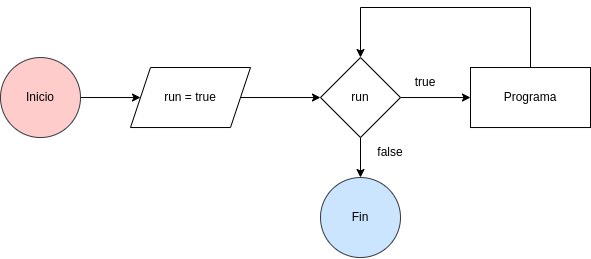
\includegraphics[width=8cm]{loop_inicio}
    \centering
        \centering
        \caption{Diagrama de Flujo del Ciclo Principal del Programa}
\end{figure}

Acá se le presenta al usuario una lista de programas disponibles y se captura la opción ingresada, este valor se evalúa con una estructura de control \emph{switch} para ejecutar cada ejercicio.

\begin{lstlisting}[style=mystyle, language=c++]
// Leer ejercicio por ejecutar
char opcion;

cout << "Ingrese una opción: ";
cin >> opcion;

cout << endl;

// Ejecutar programa con un switch
switch (opcion) {
    case 'A': {
        // Programa A
    }
    case 'B': {
        // Programa B
    }
    case 'C': {
        // Programa C
    }
    case 'D': {
        // Programa D
    }
    default: {
        // Programa de error
    }
}
\end{lstlisting}

Este se puede representar de la siguiente manera

\begin{figure}[H]
    \centering
    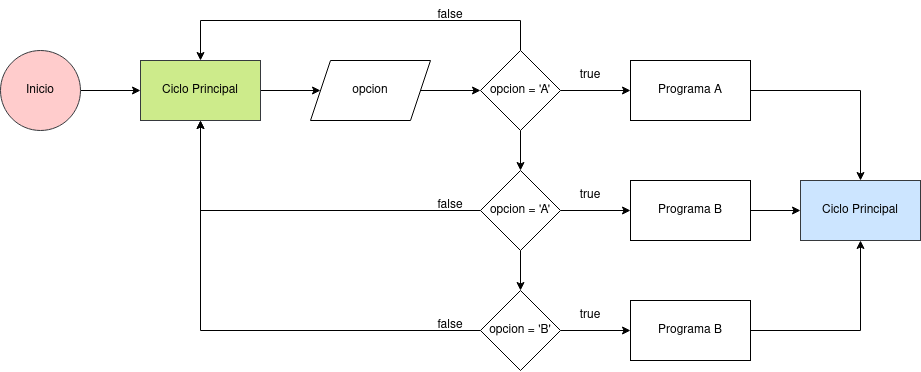
\includegraphics[width=8cm]{switch_programa}
    \caption{Diagrama de Flujo del Menú Principal}
\end{figure}

\section{Primer Programa}

El primer programa empieza capturando las 3 variables: \emph{a}, \emph{b} y \emph{c}, de tipo \emph{double} para no perder precisión al momento de calcular el área del triángulo. Estas variables son entonces evaluadas en un condicional para verificar si una de ellas es negativa o igual a 0, de ser verdad entonces se muestra el error ``¡Solo se aceptan valores positivos!'', de ser falso se continúa con otro condicional para evaluar si los valores ingresados crean un triángulo: \emph{(a + b) > c}, de ser falso se muestra el error: ``¡Los valores ingresados no crean un triángulo!''. Con estos valores ya evaluados se utiliza la \emph{fórmula de Herrón} para obtener el área del triángulo.


\begin{lstlisting}[style=mystyle, language=c++]
  cout << "Calculador de area de un triangulo" << endl;
  // Capturar el largo de cada lado
  double a, b, c;
  cout << "- Ingrese un valor para el primer  cateto: ";
  cin >> a;

  cout << "- Ingrese un valor para el segundo  cateto: ";
  cin >> b;

  cout << "- Ingrese un valor pare el tercer cateto: ";
  cin >> c;

  // Revisar si todos los valores ingresados son positivos
  if (a <= 0 || b <= 0 || c <= 0) {
    cout << "¡Solo se aceptan valores positivos!";
  } else {
    // Verificar si se ha creado un triangulo
    if ((a + b) > c) {
      cout << "Calculando resultados....";
      cout << endl;
      // Calcular Area del triangulo con la formula de Heron
      // s = (a + b + c)/2.
      // Area = √[s(s-a)(s-b)(s-c)]

      double semi_perimetro = (a + b + c) / 2;
      cout << "~ El triangulo cuenta con un semi perimetro de: "
           << semi_perimetro << " cm" << endl;

      double area = sqrt(semi_perimetro * (semi_perimetro - a) *
                         (semi_perimetro - b) * (semi_perimetro - c));
      cout << "~ El area del triangulo es: " << area << " cm cuadrados"
           << endl;
    } else {
      cout << "¡Los valores ingresados no crean un triangulo!";
    }
  }
\end{lstlisting}

Este se puede representar de la siguiente manera

\begin{figure}[H]
    \centering
    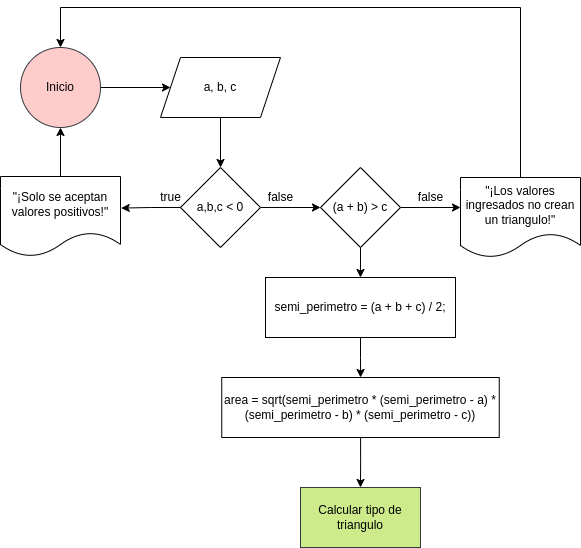
\includegraphics[width=8cm]{triangulo_area}
    \caption{Diagrama de Flujo del Calculador de Área de un Triángulo}
\end{figure}

Con el cálculo del área completo, se evalúa el tipo de triángulo con las medidas ingresadas.


\begin{lstlisting}[style=mystyle, language=c++]
// Calcular tipo de triangulo
if (a == b && a == b && b == c) {
    cout << "~ El traingulo es equilatero" << endl;
} else if (a != b && a != c && b != c) {
    cout << "~ El triangulo es escaleno" << endl;
} else {
    cout << "~ El triangulo es isoseles" << endl;
}
\end{lstlisting}

Este se puede representar de la siguiente manera

\begin{figure}[H]
    \centering
    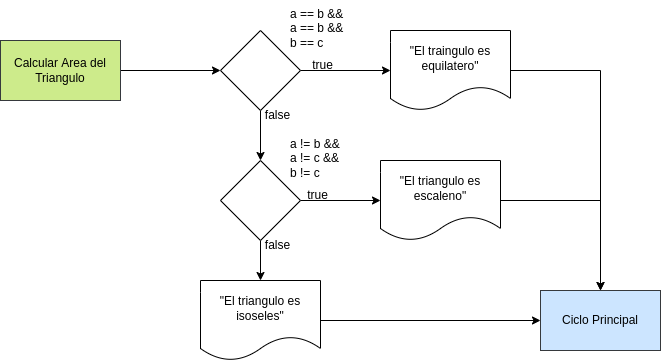
\includegraphics[width=8cm]{triangulo_tipo}
    \caption{Diagrama de Flujo del Calculador del Tipo de Triángulo}
\end{figure}

\section{Segundo Programa}

El calculador de promedio ponderado inicia solicitándole al usuario las 6 notas necesarias y su porcentaje sobre el promedio final de un estudiante, estos adicionalmente son validados para verificar si la suma de todos los porcentajes es menor a 100 o mayor a 100.

\begin{lstlisting}[style=mystyle, language=c++]
// Programa Calculador de promedio
string estudiante;
cout << "Ingrese un nombre: ";
cin >> estudiante;

float n1, n2, n3, n4, n5, n6, p1, p2, p3, p4, p5, p6, nota;

// Obtener valores
cout << "1. Ingrese un la primera nota de " + estudiante + ": ";
cin >> n1;
cout << " 1.1 Ingrese un porcentaje para la primera nota de " + estudiante + ": ";
cin >> p1;

cout << "2. Ingrese un valor para la segunda nota de " + estudiante + ": ";
cin >> n2;
cout << " 2.1 Ingrese un porcentaje para la segunda nota de " + estudiante + ": ";
cin >> p2;

cout << "3. Ingrese un valor la tercera nota de " + estudiante + ": ";
cin >> n3;
cout << " 3.1 Ingrese un porcentaje la tercera nota de " + estudiante + ": ";
cin >> p3;

cout << "4 Ingrese un valor la cuarta nota de " + estudiante + ": ";
cin >> n4;
cout << " 4.1 Ingrese un porcentaje la cuarta nota de " + estudiante + ": ";
cin >> p4;

cout << "5. Ingrese un valor la quinta nota de " + estudiante + ": ";
cin >> n5;
cout << " 5.1 Ingrese un porcentaje la quinta nota " + estudiante + ": ";
cin >> p5;

cout << "6. Ingrese un valor para la sexta nota " + estudiante + ": ";
cin >> n6;
cout << "6.1 Ingrese un porcentaje la sexta nota " + estudiante + ": ";
cin >> p6;

cout << "Validando datos..." << endl;
if ((p1 + p2 + p3 + p4 + p5 + p5) > 100 || (p1 + p2 + p3 + p4 + p5 + p6) < 100 ) {
    cout << "Los porcentajes ingresados no deben de exceder ni ser menor a un 100% ..." << endl;
} else {
    // Calcular resultados
}
\end{lstlisting}

Este fragmento de código puede ser representado de la siguiente manera

\begin{figure}[H]
    \centering
    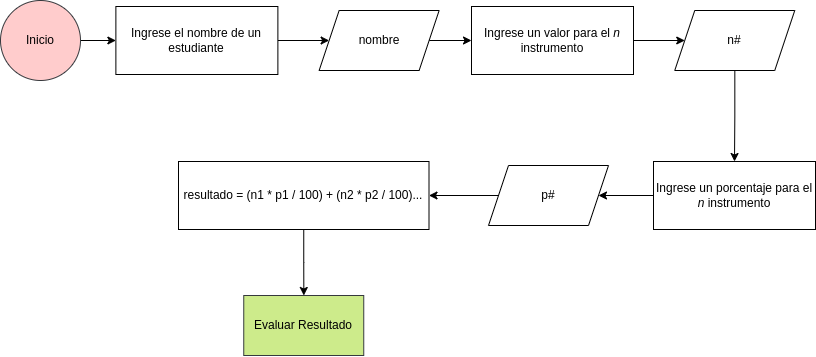
\includegraphics[width=8cm]{promedio_ponderado_calcular_resultado}
    \caption{Diagrama de Flujo del Cálculo del Promedio Ponderado}
\end{figure}

Si la verificación pasa, se calcula el resultado y se evalúa con un condicional si el estudiante ha pasado el curso con un promedio final mayor o igual a 70.

\begin{lstlisting}[style=mystyle, language=c++]
// Fuente: https://es.wikihow.com/calcular-el-promedio-ponderado
nota = (n1 * p1 / 100) + (n2 * p2 / 100) + (n3 * p3 / 100) +
       (n4 * p4 / 100) + (n5 * p5 / 100) + (n6 * p6 / 100);

cout << endl;
cout << "+ La calificación de " << estudiante << " es " << nota << endl;

// Evaluar resultado
if (nota >= 70) {
  cout << estudiante << " ha aprobado el curso de programación!" << endl;
} else {
  cout << estudiante << " ha reprobado el curso de programación" << endl;
}
\end{lstlisting}

Este fragmento se puede representar de la siguiente manera.

\begin{figure}[H]
    \centering
    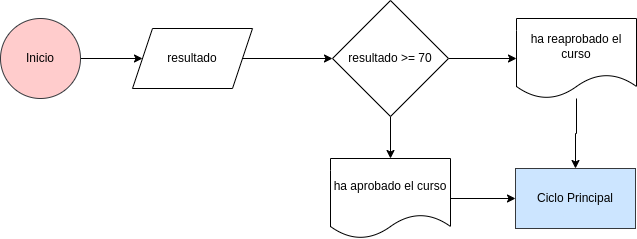
\includegraphics[width=8cm]{promedio_ponderado_salida}
    \caption{Diagrama de Flujo del Resultado Final del Promedio Ponderado}
\end{figure}

\section{Tercer Programa}

El contador de dígitos solícito el ingreso de un número, este número es en realidad capturado en una variable de tipo \emph{String} para obtener su largo con la propiedad \emph{length}. Esta propiedad es usada para validar la cantidad de dígitos con la función \emph{length}

\begin{lstlisting}[style=mystyle, language=c++]
  cout << "Contador de dígitos." << endl;
  string numero;

  // Capturar un número
  cout << "Ingrese un numero de máximo 4 dígitos:";
  cin >> numero;

  // Con la funcion length es posible obtner el largo de una cadena de text
  int largo = numero.length();
  if (largo <= 4) {
    // Calcular cantidad de dígitos
  } else {
    cout << "¡El numero ingreado no es valido!" << endl;
  }
  break;
\end{lstlisting}

Este fragmento de código se puede representar de la siguiente manera.

\begin{figure}[H]
    \centering
    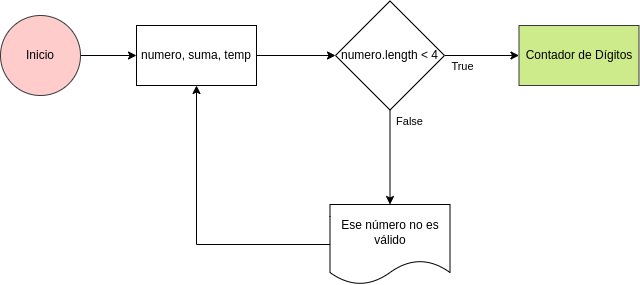
\includegraphics[width=8cm]{contador_digitos_validacion}
    \caption{Diagrama de la Validación del Programa Contador de Dígitos}
\end{figure}

Adicionalmente se usa esta función para crear un ciclo \emph{for} con el cual se itera sobre cada carácter para poder sumarlo a una variable acumuladora llamada \emph{suma}, cabe a destacar el uso de la función \emph{stoi}, la cual permite convertir valores de tipo \emph{String} a valores de tipo numerales \emph{int} así como el uso de una variable ``temporal'' para guardar el valor actual del carácter por sumar.

\begin{lstlisting}[style=mystyle, language=c++]
for (int i = 0; i < largo; i++) {
  // Guardar el número actual en el ciclo
  // '1[2]3' -> numero_actual = 2
  numero_actual = numero[i];
  // Convertir de texto a numero
  // '2' -> 2
  // Puede causar un error si se ingresa una letra!
  // 'o' -> error
  suma_final = suma_final + stoi(numero_actual);
}
\end{lstlisting}

Este fragmento de código se puede representar de la siguiente manera.

\begin{figure}[H]
    \centering
    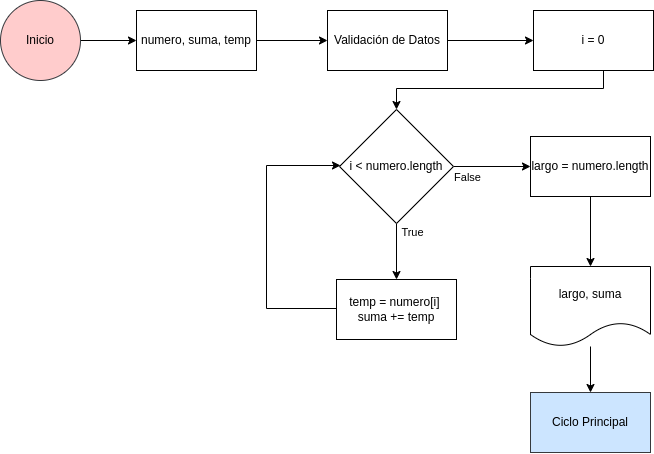
\includegraphics[width=8cm]{contador_digitos_ciclo}
    \caption{Diagrama de Flujo del Ciclo \emph{for} del Programa Contador de Dígitos}
\end{figure}

\section{Limitador de Intentos}

En el capítulo dedicado a cada programa se ha estado omitiendo, el limitador de intentos máximos en caso de que el usuario ingrese una opción inválida al momento de seleccionar un programa por ejecutar, esto es logrado mediante una variable \emph{intentos}, la cual es reducida cada vez que el usuario ingresa un valor no esperado en el menú principal para que cuando este llegue a 3, se cierre el ciclo principal del programa poniendo el valor de la variable booleana \emph{run} en falso.

\begin{lstlisting}[style=mystyle, language=c++]
// Reducir la cantidad de intentos
intentos = intentos - 1;
cout << "Esa no es una opción valida... Tiene " << intentos <<  "intentos restantes..." << endl; 
if (intentos == 0) {
    cout << "Se ha llegado al limite de intentos máximos, cerrando programa.." << endl;
    run = false;
}
\end{lstlisting}

Este fragmento de código se puede representar de la siguiente manera.

\begin{figure}[H]
    \centering
    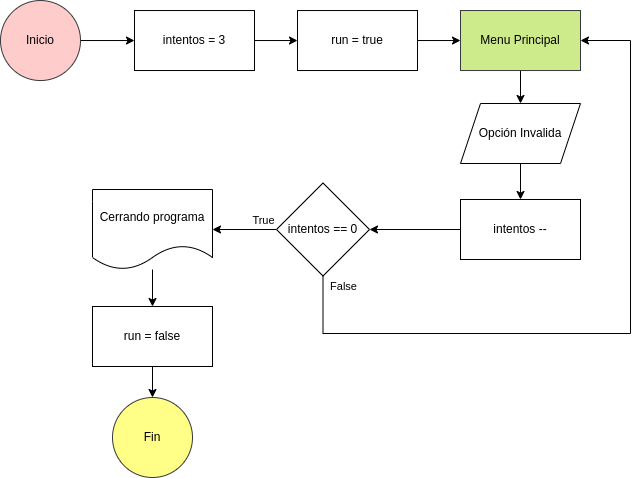
\includegraphics[width=8cm]{limitador_intentos_salida}
    \caption{Diagrama de Flujo del Programa de Salida}
\end{figure}

Cabe a destacar que este contador es restaurado cada vez que el usuario ingresa correctamente una opción presentada en el menú principal.

\begin{lstlisting}[style=mystyle, language=c++]
const int intentos_maximos = 3;
// Contador de intentos restantes
int intentos = intentos_maximos;

// Leer ejercicio por ejecutar
char opcion;

cout << "Ingrese una opción: ";
cin >> opcion;

cout << endl;

// Ejecutar programa con un switch
switch (opcion) {
    case 'A': {
        // Programa A
        // Reiniciar la cantidad de intentos
        intentos = intentos_maximos;
    }
    case 'B': {
        // Programa B
        // Reiniciar la cantidad de intentos
        intentos = intentos_maximos;
    }
    case 'C': {
        // Programa C
        // Reiniciar la cantidad de intentos
        intentos = intentos_maximos;
    }
    case 'D': {
        // Programa D
        // Reiniciar la cantidad de intentos
        intentos = intentos_maximos;
    }
    default: {
        // Programa de error
        // Reiniciar la cantidad de intentos
        intentos = intentos_maximos;
    }
}
\end{lstlisting}
\begin{figure}[H]
    \centering
    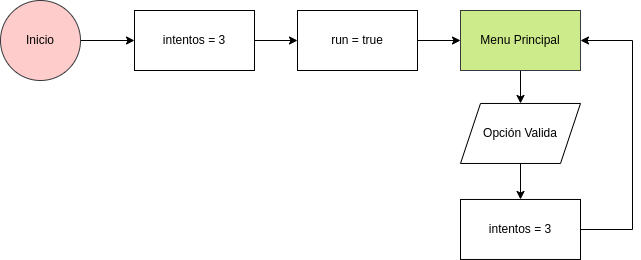
\includegraphics[width=8cm]{limitador_intentos_reinicio}
    \caption{Diagrama de Flujo del Limitador de Intentos}
\end{figure}

\section{Programa de Salida}

El programa de salida corresponde a un simple condicional que solicita confirmación del usuario para terminar la ejecución, si se confirma la salida del programa entonces se cambia el valor de la variable \emph{run} a falso y se cierra el ciclo principal del programa.

\begin{lstlisting}[style=mystyle, language=c++]
  char salir;
  cout << "¿Desea terminar el programa? [s/n]: ";
  cin >> salir;

  switch (salir) {
      case 's': {
        cout << "Terminando programa..." << endl;
        run = false;
        break;
      }
      case 'n': {
        // No hacer nada
        break;
      }
      default: {
        cout << "¡Esa no es una opción valida!" << endl;
      }
  }
\end{lstlisting}

Este fragmento de código se puede representar de la siguiente manera.

\begin{figure}[H]
    \centering
    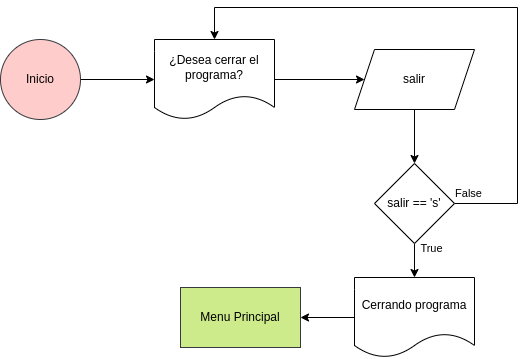
\includegraphics[width=8cm]{programa_salida}
    \caption{Diagrama de Flujo del Programa de Salida}
\end{figure}

\end{document}
